%%%%%%%%%%%%%%%%%%%%%%%%%%%%%%%%%%%%%%%%%
%
% Classicthesis Typographic Thesis
% LaTeX Template
% Version 1.1 (4/8/12)
%
% This template has been downloaded from:
% http://www.LaTeXTemplates.com
%
% Original author:
% André Miede (http://www.miede.de)
%
% License:
% CC BY-NC-SA 3.0 (http://creativecommons.org/licenses/by-nc-sa/3.0/)
%
%%%%%%%%%%%%%%%%%%%%%%%%%%%%%%%%%%%%%%%%%

%----------------------------------------------------------------------------------------
%	PACKAGES AND OTHER DOCUMENT CONFIGURATIONS
%----------------------------------------------------------------------------------------

\documentclass[
				twoside,openright,titlepage,numbers=noenddot,headinclude,%1headlines,
                footinclude=true,cleardoublepage=empty,
                BCOR=5mm,paper=letter,fontsize=9pt, % Binding correction, paper type and font size
                estonian,swedish,spanish,american, % Languages
                ]{scrreprt} 
                
%%%%%%%%%%%%%%%%%%%%%%%%%%%%%%%%%%%%%%%%%
% Configuration File
%
% The main lines to change in this file are in the DOCUMENT VARIABLES
% section, the rest of the file is for advanced configuration.
%
%%%%%%%%%%%%%%%%%%%%%%%%%%%%%%%%%%%%%%%%%

\PassOptionsToPackage{dottedtoc,eulerchapternumbers,pdfspacing,subfig,beramono,eulermath,parts}{classicthesis}

\newcommand{\myTitle}{Estonian Textbook\xspace}
\newcommand{\mySubtitle}{Traducci\'on no-oficial al espa\~nol \xspace}
\newcommand{\myName}{Juhan Tuldava \dag \xspace}
\newcommand{\myTime}{2013\xspace}
\newcommand{\myVersion}{versi\'on 0.00\xspace}

%----------------------------------------------------------------------------------------
%	USEFUL COMMANDS
%----------------------------------------------------------------------------------------

\newcommand{\ie}{i.\,e.}
\newcommand{\Ie}{I.\,e.}
\newcommand{\eg}{e.\,g.}
\newcommand{\Eg}{E.\,g.} 
\newcommand{\bemph}{\textbf}
\newcounter{dummy} % Necessary for correct hyperlinks (to index, bib, etc.)
\providecommand{\mLyX}{L\kern-.1667em\lower.25em\hbox{Y}\kern-.125emX\@}

%----------------------------------------------------------------------------------------
%	PACKAGES
%----------------------------------------------------------------------------------------

\usepackage{textcomp} % Used for special characters

%------------------------------------------------

\usepackage{lipsum} % Used for inserting dummy 'Lorem ipsum' text into the template

%------------------------------------------------
 
%\PassOptionsToPackage{latin9}{inputenc} % latin9 (ISO-8859-9) = latin1+"Euro sign"
\usepackage[utf8]{inputenc}
 
 %------------------------------------------------

%\PassOptionsToPackage{ngerman,american}{babel}  % Change this to your language(s)
% Spanish languages need extra options in order to work with this template
%\PassOptionsToPackage{spanish,es-lcroman}{babel}
\usepackage[swedish, estonian, spanish]{babel}
 
 %------------------------------------------------

\PassOptionsToPackage{T1}{fontenc} % T2A for cyrillics
\usepackage{fontenc}

%------------------------------------------------

\usepackage{xspace} % To get the spacing after macros right

%------------------------------------------------

\usepackage{mparhack} % To get marginpar right

%------------------------------------------------

\usepackage{fixltx2e} % Fixes some LaTeX stuff 

%------------------------------------------------

\PassOptionsToPackage{smaller}{acronym} % Include printonlyused in the first bracket to only show acronyms used in the text
\usepackage{acronym} % nice macros for handling all acronyms in the thesis

%------------------------------------------------

\PassOptionsToPackage{pdftex}{graphicx}
\usepackage{graphicx} 
  
%----------------------------------------------------------------------------------------
%	FLOATS: TABLES, FIGURES AND CAPTIONS SETUP
%----------------------------------------------------------------------------------------

\usepackage{tabularx} % Better tables
\setlength{\extrarowheight}{3pt} % Increase table row height
\newcommand{\tableheadline}[1]{\multicolumn{1}{c}{\spacedlowsmallcaps{#1}}}
\newcommand{\myfloatalign}{\centering} % To be used with each float for alignment
\usepackage{caption}
\captionsetup{format=hang,font=small}
\usepackage{subfig}

%----------------------------------------------------------------------------------------
%	HYPERREFERENCES
%----------------------------------------------------------------------------------------

\PassOptionsToPackage{pdftex,hyperfootnotes=false,pdfpagelabels}{hyperref}
\usepackage{hyperref}  % backref linktocpage pagebackref
\pdfcompresslevel=9
\pdfadjustspacing=1

\hypersetup{
% Uncomment the line below to remove all links (to references, figures, tables, etc)
%draft, 
colorlinks=true, linktocpage=true, pdfstartpage=3, pdfstartview=FitV,
% Uncomment the line below if you want to have black links (e.g. for printing black and white)
%colorlinks=false, linktocpage=false, pdfborder={0 0 0}, pdfstartpage=3, pdfstartview=FitV, 
breaklinks=true, pdfpagemode=UseNone, pageanchor=true, pdfpagemode=UseOutlines,
plainpages=false, bookmarksnumbered, bookmarksopen=true, bookmarksopenlevel=1,
hypertexnames=true, pdfhighlight=/O, urlcolor=webbrown, linkcolor=RoyalBlue, citecolor=webgreen,
%------------------------------------------------
% PDF file meta-information
pdftitle={\myTitle},
pdfauthor={\myName},
pdfsubject={},
pdfkeywords={},
pdfcreator={pdfLaTeX},
pdfproducer={LaTeX with hyperref and classicthesis}
%------------------------------------------------
}   

%----------------------------------------------------------------------------------------
%	BACKREFERENCES
%----------------------------------------------------------------------------------------

\usepackage{ifthen} % Allows the user of the \ifthenelse command
\newboolean{enable-backrefs} % Variable to enable backrefs in the bibliography
\setboolean{enable-backrefs}{false} % Variable value: true or false

\newcommand{\backrefnotcitedstring}{\relax} % (Not cited.)
\newcommand{\backrefcitedsinglestring}[1]{(Cited on page~#1.)}
\newcommand{\backrefcitedmultistring}[1]{(Cited on pages~#1.)}
\ifthenelse{\boolean{enable-backrefs}} % If backrefs were enabled
{
\PassOptionsToPackage{hyperpageref}{backref}
\usepackage{backref} % to be loaded after hyperref package 
\renewcommand{\backreftwosep}{ and~} % separate 2 pages
\renewcommand{\backreflastsep}{, and~} % separate last of longer list
\renewcommand*{\backref}[1]{}  % disable standard
\renewcommand*{\backrefalt}[4]{% detailed backref
\ifcase #1 
\backrefnotcitedstring
\or
\backrefcitedsinglestring{#2}
\else
\backrefcitedmultistring{#2}
\fi}
}{\relax} 

%----------------------------------------------------------------------------------------
%	AUTOREFERENCES SETUP
%	Redefines how references in text are prefaced for different 
%	languages (e.g. "Section 1.2" or "section 1.2")
%----------------------------------------------------------------------------------------

\makeatletter
\@ifpackageloaded{babel}
{
\addto\extrasamerican{
\renewcommand*{\figureautorefname}{Figure}
\renewcommand*{\tableautorefname}{Table}
\renewcommand*{\partautorefname}{Part}
\renewcommand*{\chapterautorefname}{Chapter}
\renewcommand*{\sectionautorefname}{Section}
\renewcommand*{\subsectionautorefname}{Section}
\renewcommand*{\subsubsectionautorefname}{Section}
}
\addto\extrasngerman{
\renewcommand*{\paragraphautorefname}{Absatz}
\renewcommand*{\subparagraphautorefname}{Unterabsatz}
\renewcommand*{\footnoteautorefname}{Fu\"snote}
\renewcommand*{\FancyVerbLineautorefname}{Zeile}
\renewcommand*{\theoremautorefname}{Theorem}
\renewcommand*{\appendixautorefname}{Anhang}
\renewcommand*{\equationautorefname}{Gleichung}
\renewcommand*{\itemautorefname}{Punkt}
}
\providecommand{\subfigureautorefname}{\figureautorefname} % Fix to getting autorefs for subfigures right
}{\relax}
\makeatother

%----------------------------------------------------------------------------------------

\usepackage{classicthesis} 

%---------------------------------------------------------------------------------------- % File which contains all the document configurations and packages

\begin{document}

\frenchspacing % Reduces space after periods to make text more compact

\raggedbottom % Makes all pages the height of the text on that page

\selectlanguage{spanish} % Default language

\pagenumbering{roman} % Roman page numbering prior to the start of the thesis content (i, ii, iii, etc)

\pagestyle{plain} % Suppress headers for the pre-content pages

%----------------------------------------------------------------------------------------
%	PRE-CONTENT BOOK PAGES
%----------------------------------------------------------------------------------------

% Title Page

\begin{titlepage}

\begin{addmargin}[-1cm]{-3cm}
\begin{center}
\large

\hfill
\vfill

\begingroup
\color{MidnightBlue}\spacedallcaps{\myTitle} \\ \bigskip % Book title
\endgroup

\spacedlowsmallcaps{\myName} % Author's name

\vfill

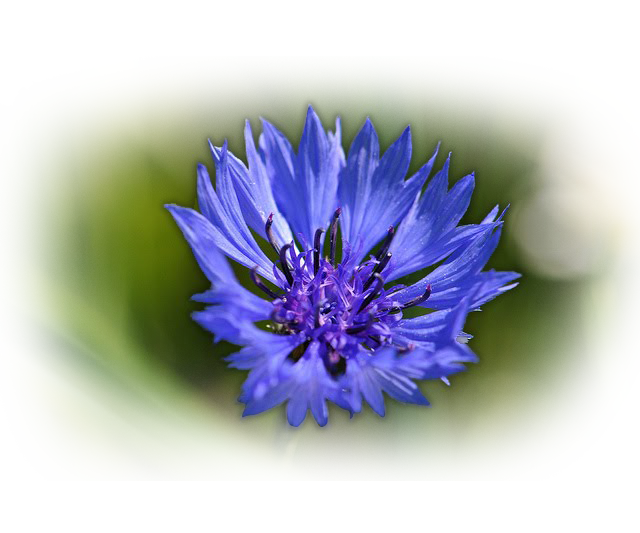
\includegraphics[width=10cm]{img/Estonian_Flower.png} \\ \medskip % Picture

\mySubtitle \\ \medskip % Book subtitle

\myTime\ -- \myVersion % Time and version

\vfill

\end{center}
\end{addmargin}

\end{titlepage}
 

% Back of the title page

\thispagestyle{empty}

\hfill

\vfill

\noindent\myName: \textit{\myTitle,} \mySubtitle, %\myDegree, 
\textcopyright\ \myTime 

\cleardoublepage% Dedication

\thispagestyle{empty}
\refstepcounter{dummy}

\pdfbookmark[1]{Dedicatoria}{Dedicatoria} % Bookmark

\vspace*{3cm}

\begin{center}
Ükskord me võidame, niikuinii! \\ \medskip
--- Heinz Valk
\end{center}

\medskip

\begin{center}
Este libro está dedicado a todas aquellas personas que deseen sumergirse en este fascinante y hermoso idioma.
\end{center}
 

\cleardoublepage% Acknowledgements

\pdfbookmark[1]{Agradecimientos}{Agradecimientos} % Bookmark 

\chapter*{Agradecimientos} 

\lipsum[7]

Probanfo las citas \cite{bentley:1999}. \\
Probanfo las citas \cite{bringhurst:2002} . \\
Probanfo las citas \cite{cormen:2001} . \\
Probanfo las citas \cite{dueck:trio} . \\
Probanfo las citas \cite{knuth:1976} . \\
Probanfo las citas \cite{knuth:1974} . \\
Probanfo las citas \cite{sommerville:1992} . \\

%\noindent Más agradecimientos aquí \\


\cleardoublepage% License

\thispagestyle{empty}
\refstepcounter{dummy}

\pdfbookmark[1]{Licencia}{Licencia} % Bookmark

\vspace*{3cm}

\begin{center}
 
\includegraphics[width=3cm]{img/by-nc-sa.pdf}\\ \bigskip
 El presente libro se distribuye con licencia \href{http://creativecommons.org/licenses/by-nc-sa/3.0/}{Creative Commons BY-NC-SA}
\end{center}

\pagestyle{scrheadings} % Show chapter titles as headings

\cleardoublepage% Table of Contents - List of Tables/Figures/Listings and Acronyms

\refstepcounter{dummy}

\pdfbookmark[1]{\contentsname}{tableofcontents} % Bookmark name visible in a PDF viewer

\setcounter{tocdepth}{2} % Depth of sections to include in the table of contents - currently up to subsections

\setcounter{secnumdepth}{3} % Depth of sections to number in the text itself - currently up to subsubsections

\manualmark
\markboth{\spacedlowsmallcaps{\contentsname}}{\spacedlowsmallcaps{\contentsname}}
\tableofcontents 
\automark[section]{chapter}
\renewcommand{\chaptermark}[1]{\markboth{\spacedlowsmallcaps{#1}}{\spacedlowsmallcaps{#1}}}
\renewcommand{\sectionmark}[1]{\markright{\thesection\enspace\spacedlowsmallcaps{#1}}}

\clearpage

\begingroup 
\let\clearpage\relax
\let\cleardoublepage\relax
\let\cleardoublepage\relax
                   
\endgroup

\cleardoublepage
 

\pagenumbering{arabic} % Arabic page numbering for thesis content (1, 2, 3, etc)

\cleardoublepage% Foreword

\pdfbookmark[1]{Foreword}{Foreword} % Bookmark name visible in a PDF viewer

\chapter*{Prólogo} % Foreword name

Durante siglos, los estonios han tenido contacto cercano con otras nacionalidades que viven en la zona del Mar Báltico al noreste de Europa. Entre las dos Guerras Mundiales (cuando Estonia era independiente), se fortalecieron los contactos políticos, económicos y culturales con los países vecinos. Incluso los contactos personales se desarrollaron, en gran medida, debido al turismo. Los mismos procesos se haces aún más evidentes hoy en día, después de que Estonia recuperara su independencia de la Unión Soviética en 1991.\\

A finales de la Segunda Guerra Mundial, decenas de miles de estonios huyeron a Suecia y Alemania. Muchos de ellos se instalaron en los Estados Unidos de América, Canadá y Australia. Fueron recibidos con amistad y entendimiento en los países donde buscaron refugio. En sus actividades laborales y de ocio diarios, los estonios se adaptaron bien a la vida en otros países, y la mayoría de ellos son ahora ciudadanos de sus nuevas patrias.\\

Los estonios en el extranjero no han olvidado su origen o su lengua. Quieren preservar su patrimonio cultural y mantener sus tradiciones. La colección de folclore de Estonia, por ejemplo, es uno de los más grandes del mundo, y los estonios en el extranjero con orgullo cuentan a sus hijos y amigos sobre el legendario héroe cuyas hazañas se registran en el épico folclore Kalevipoeg. Hay incluso una extensa y muy rica variedad de literatura estonia moderna, aunque poco de ella ha sido traducida a otros idiomas aún. Músicos y cantantes de Estonia son excepcionales, y grandes festivales en su patria así como en el extranjero reúnen a miles de miembros del coro, bailarines folclóricos, y gimnastas rítmicos para ganar fama por sus actuaciones. Anticuadas artesanías estonias también han llamado la atención - particularmente las artes textiles, cuero, madera y orfebrería. Muchos artistas y estudiosos contemporáneos han ganado reconocimiento internacional, por trabajos relacionados o inspirados por las viejas tradiciones y nuevos desarrollos en Estonia.\\

La lengua estonia pertenece a la familia ugrofinesa, junto con el finés, el húngaro, las lenguas sami (lapón), y un número de otras lenguas habladas por los pueblos dispersos en el norte de Rusia. Las lenguas de los pueblos cercanos - ruso, letón, lituano, sueco - se encuentran en un grupo diferente, llamada la familia indoeuropea. El inglés también se encuentra en esta última familia, lo que significa que su estructura difiere en importantes aspectos de la lengua estonia. Sin embargo, no es tan difícil para una persona de habla inglesa aprender estonio como generalmente se cree.\\

Este libro está destinado principalmente para los estadounidenses y otros hablantes del inglés que, por diversas razones, están interesados en el idioma estonio. En la preparación de este libro, sin embargo, el autor también tuvo en cuenta la generación más joven de los estonios residentes en el extranjero, sin la oportunidad de aprender la gramática del estonio en las escuelas a las que asisten.\\

El libro se puede utilizar para el estudio independiente, pero para un aprendizaje óptimo, se recomienda la ayuda de una persona de habla estonia, sobre todo al principio. En caso de que el libro se utilice en un curso, el instructor puede cambiar el orden de los temas o añadir más ejercicios según sea necesario.\\

El libro contiene 40 lecciones, cada una de las cuales tiene seis secciones: gramática, texto (selección de lectura), vocabulario, ejercicios (diseñado para reforzar el aprendizaje tanto de gramática como de vocabulario), expresiones (elegidas acorde a la gramática del capítulo en mente, y a menudo agrupados por tema), y las respuestas a los ejercicios.\\

En las secciones de gramática, el autor ha tratado de presentar las principales características de la gramática estonia de la forma más sencilla posible. Para hacer las cosas más claras, las comparaciones con las reglas de la gramática inglesa se hacen a menudo.\\

Aquellos que no tienen deseo ni tiempo para un estudio profundo de la gramática estonia pero que desean ampliar su repertorio de frases coloquiales y palabras comunes encontrará el tema de las expresiones de cada lección (Saludos y Agradecimientos, Comidas y Bebidas, Tiempo, Clima, Correspondencias, Enfermedad , Oficio, etc.) listadas en la tabla de contenidos. El índice también enumera los temas tratados en las lecturas y las listas de expresiones.\\

Las selecciones de lectura, mayormente composiciones originales hechas por el autor, están diseñadas para reforzar los puntos de la gramática. Las cursivas se utilizan para identificar las palabras o frases que ilustran las formas gramaticales presentadas en la misma lección. Al mismo tiempo, el autor ha tratado de cubrir un amplio rango de temas y situaciones para construir el vocabulario del alumno tanto como sea posible para una conversación regular.\\

Al final del libro se incluye un diccionario general de Estonia-Inglés, con todos los términos presentados en la lista de vocabulario de cada capítulo y otras palabras comunes. Para la traducción de palabras del inglés al estonio, el estudiante necesitará un diccionario Inglés-Estonio. Una breve revisión de los términos gramaticales también se presenta al final. El índice consta de dos partes, con listados alfabéticos separados en términos gramaticales y temas de conversación.\\

La idea de escribir un libro sobre el estonio se presentó en el verano de 1960 en el curso de la Escuela de Continuación Estonia (Estniska Folkhögskolan) en Gimo, Suecia, donde el autor enseñó estonio por varios años y por lo mismo obtuvo la perspicacia sobre las dificultades de instruir a los jóvenes sin previo estudio de la gramática estonia.\\

La fuente de inspiración fue ombudsman Nils Hellstrom, y estoy muy agradecido con él, no sólo por surgir con la idea de este libro, sino también por organizar su primera publicación (en 1962) a través de Bokförlaget Medborgarskolan. También deseo expresar mis agradecimientos al director Henry Jarild, por su cooperación y ayuda en relación con la publicación original de este libro.\\

Quiero expresar un especial agradecimiento a Gita Aasmaa y Tarmo Oja, no sólo por proporcionar diversas formas de asistencia técnica, sino también por contribuir puntos de vista muy valiosos y sugerencias con respecto al contenido del libro.\\

Estoy especialmente agradecido con el profesor Ain Haas por asumir y llevar a cabo extremadamente bien la enorme tarea de traducir y actualizar el libro de esta edición.\\

\hfill \textit{Juhan Tuldava}

\hfill Tartu, Estonia			

\vfill
 

\cleardoublepage% Translation Notes

\pdfbookmark[1]{Translation}{Translation} % Bookmark name visible in a PDF viewer

\chapter*{Nota del Traductor} % Translation Notes name

Varios libros están disponibles para las personas que desean estudiar el idioma Estonio. Cualquier persona seria en el asunto no debería pasar por alto el trabajo del profesor Tuldava. En el esfuerzo por mejorar mi dominio del estonio, no encontré nada más valioso que su libro. Es verdaderamente impresionante en su claridad, rigurosidad y lógica de progresión. Provee un riguroso curso de instrucciones, equivalente a dos años universitarios, pero tiene muchos giros interesantes e incluso toques humorísticos que hacen las lecciones agradables.\\

Después de descubrir el libro durante un viaje de investigación a Suecia, llegué a sentir que merecía una distribución mucho más amplia. Como un Estonio nacido en Suecia y criado en los Estados Unidos, con fluidez en los tres idiomas, me encontré en una buena posición para preparar una versión en Inglés de este excelente libro, para el beneficio de los familiares y amigos en los EE.UU. que no pudieron hacer uso de la versión sueca. Debido a su apoyo, así como un creciente número de solicitudes de otras partes, he decidido hacer mi traducción a disposición de un público más amplio. El creciente interés por la lengua entre todo tipo de personas que no tienen una conexión ancestral con el país refleja la nueva situación de Estonia como país europeo vanguardista haciendo grandes avances para superar el legado de la ocupación soviética.\\

La versión en Inglés es básicamente la misma que la versión sueca, pero se hicieron algunos cambios en la preparación de esta traducción. Sustituí referencias a nombres de Estados Unidos, ubicaciones, divisas, etc. de muchas de las originales suecas, y me tomé la libertad de añadir algunas expresiones que había encontrado en mi análisis de diccionarios y literatura de Estonia. Se han quitado puntos de la gramática aplicable solo a la lengua sueca, y han sido agregados nuevos comentarios sobre la gramática del Inglés. Para que sea más fácil utilizar el libro para el estudio independiente, he desarrollado un conjunto más completo de respuestas a los ejercicios y ampliado el glosario.\\

Durante una temporada como profesor visitante de sociología en la Universidad de Tartu en la primavera de 1993, me aproveché de la oportunidad para reunirme con el profesor Tuldava, quien recientemente se retiró como jefe del Departamento de Lenguas Germánicas. Hablamos sobre cómo actualizar y mejorar la publicación original sueca. Sus sugerencias - incluyendo algunos nuevos puntos sobre gramática que reflejan el uso cambiante en Estonia - se han incorporado en la versión.\\

Me gustaría expresar un especial agradecimiento al profesor Tuldava y a mi madre, Elly (Ratas) Haas, por comprobar cuidadosamente el manuscrito en varias etapas y ofrecer muchas sugerencias útiles.\\

Es con gran placer y orgullo que ofrezco esta traducción del libro del profesor Tuldava, a todos aquellos que busquen una llave para abrir los misterios del idioma Estonio y abrir la puerta a un mundo oculto de fascinante folclore, buena literatura y agradables conversaciones. Hay más de un millón de hablantes del idioma Estonio en el mundo hoy en día, y es mi mayor anelo que algunos más se animen a unirse a sus filas como resultado de este libro.\\

\hfill \textit{Ain Haas}

\hfill Indianapolis, USA.			

\vfill
 

\cleardoublepage% Abreviations & Symbols

\pdfbookmark[1]{Abreviaturas y Símbolos}{Abreviaturas y Simbolos} % Bookmark name visible in a PDF viewer

\chapter*{Abreviaturas y Símbolos} % Abreviations & Symbols name

\begin{tabular}{ l l }
	\begin{tabular}{ l c l }
	abbr.	& = & abreviatura \\
	abess.	& = & abesivo \\
	abl.	& = & ablativo \\
	adess.	& = & adesivo \\
	adj.	& = & adjetivo \\
	adv.	& = & adverbio \\
	all.	& = & alativo \\
	comit.	& = & comitativo \\
	comp.	& = & comparativo \\
	conj.	& = & conjunción \\
	cont.	& = & continuado \\
	dim.	& = & diminutivo \\
	e.g.	& = & por ejemplo \\
	elat.	& = & elativo \\
	emph.	& = & enfático \\
	etc.	& = & etcétera \\
	gen.	& = & genitivo \\
	i.e.	& = & en esencia \\
	ill.	& = & ilativo \\
	imper.	& = & imperativo \\
	imperf.	& = & imperfecto \\
	indecl.	& = & indeclinable \\
	iness.	& = & inesivo \\
	inf.	& = & infinitivo \\
	interj.	& = & interjección
	\end{tabular}
&
	\begin{tabular}{ l c l }
	lit.	& = & literalmente \\
	n.		& = & sustantivo \\
	neg.	& = & negativo \\
	nom.	& = & nominativo \\
	num.	& = & número \\
	part.	& = & partitivo \\
	partic.	& = & participio \\
	pass.	& = & pasivo \\
	perf.	& = & perfecto \\
	pers.	& = & persona \\
	pl.		& = & plural \\
	postp.	& = & posposición \\
	prep.	& = & preposición \\
	pres.	& = & presente \\
	pron.	& = & pronombre \\
	refl.	& = & reflexivo \\
	sing.	& = & singular \\
	superl.	& = & superlativo \\
	term.	& = & terminativo \\
	transl.	& = & translativo \\
	v.		& = & verbo \\
	v.i.	& = & verbo intransitivo \\
	vs.		& = & versus \\
	v.t.	& = & verbo transitivo
	\end{tabular}
\end{tabular}\\ \bigskip

\begin{tabular}{ l p{10cm} }
	\textasciiacute & indica que la tensión está en una sílaba dada, en contraste con el patrón habitual de hacer hincapié en la primera sílaba. \\
	\textasciigrave & indica un sonido extra largo (tercer grado) en la sílaba que sigue. \\
	\textquotesingle & indica palatalización de consonante. \\
	\S & significa sección.
\end{tabular}		

\vfill
 

\cleardoublepage 

%----------------------------------------------------------------------------------------
%	BOOK CONTENT - LESSONS
%----------------------------------------------------------------------------------------

\ctparttext{Dentro de esta primera parte se expondrán la introducción y las 40 lecciones principales que constituyen el fuerte del libro. Es altamente recomendable realizar los ejercicios propuestos al final de cada lección, pues ayuda a decantar la teoría expuesta en la misma y proporciona un escenario real de aplicación.} 

\part{Manual Estonio} 

% Introduction

\pdfbookmark[1]{Introduction}{Introduction} % Bookmark name visible in a PDF viewer

\chapter*{Introducción} % Introduction name

\begin{enumerate}
	\item El alfabeto estonio básico consta de 23 letras en el siguiente orden:
	\begin{center}
	\begin{otherlanguage}{estonian}
		\textbf{a b c d e g h i j k l m n o p r s t u v õ ä ö ü}
	\end{otherlanguage}
	\end{center}

	Hay otras 9 letras que aparecen en las palabras extranjeras. Las letras \textbf{c q w x y} se encuentran sólo en los nombres extranjeros, como César, Don Quijote, Xantippe, Nueva York. Las letras \foreignlanguage{estonian}{\textbf{f š z ž}} se encuentran en las nuevas palabras prestadas de otros idiomas: \foreignlanguage{estonian}{film, šokolaad, zooloog, žurnaal}. El orden del alfabeto completo es:
	\begin{center}
	\begin{otherlanguage}{estonian}
		\textbf{a b c d e f g h i j k l m n o p q r s š z ž t u v w õ ä ö ü x y}
	\end{otherlanguage}
	\end{center}

	\item En cuanto a la pronunciación, tenga en cuenta lo siguiente:

	\section*{\Large{Vocales}}

	Las vocales \textbf{a e i o u} se pronuncian exactamente igual que en español, sin embargo la fonética de las vocales \foreignlanguage{estonian}{\textbf{ä õ ö ü}} puede presentar una gran dificultad. Es por eso que se recomienda escuchar la pronunciación de las vocales más que leer una descripción. El siguiente \href{http://www.youtube.com/watch?v=GfxrR45yA6I}{video}\footnote{http://www.youtube.com/watch?v=GfxrR45yA6I} presenta de una forma precisa y concisa las vocales del estonio.\\

	Noten que las tres vocales \foreignlanguage{estonian}{\textbf{õ ö ü}} son bastante similares. Una forma de comparar la pronunciación de estas tres vocales es considerar a \foreignlanguage{estonian}{\textbf{õ}} como la pronunciación de una \textbf{o} y una \textbf{u} al mismo tiempo. Para \foreignlanguage{estonian}{\textbf{ö}} es exactamente lo mismo, pero predomina más la \textbf{o}. De manera análoga, para \foreignlanguage{estonian}{\textbf{ü}} predomina más la \textbf{u}.\\

	Si bien ésta es una descripción bastante burda de cómo pronunciar las tres vocales anteriores, da una idea general desde la cual partir.

 	\section*{\Large{Consonantes}}

 	\begin{tabular}{ r p{9cm} }

 	\textbf{z} & se pronuncia igual que en inglés.\\[0.5cm]

 	\textbf{j} & se pronuncia como la letra \textbf{y} en la palabra `Maya'.\\[0.5cm] 

 	\textbf{h} & si está al principio de una palabra el sonido es muy débil, casi un silencio. Si está en medio de dos vocales se pronuncia como la \textbf{j} en la interjección coloquial `¡Ajá!', y si se encuentra antes de una consonante o al final de una palabra su pronunciación se torna más como una exhalación muy suave, haciendo amagos en formar una \textbf{j}.\\[0.5cm]

 	\textbf{b d g} & son sordas y ligeramente más suaves que las letras \textbf{p t k} del español, respectivamente.\\[0.5cm]

 	\textbf{p t k} & son sordas y ligeramente más fuertes que en español. Un sonido más duradero y ligeramente más potente se da en el caso de tener consonantes dobles \textbf{pp tt kk}\\[0.5cm]  

 	\foreignlanguage{estonian}{\textbf{š}} & equivale a la combinación \textbf{sh}, como en la palabra inglesa `english'.\\[0.5cm]

 	\foreignlanguage{estonian}{\textbf{ž}} & es como la \textbf{s} en la palabra inglesa `treasure' o como la \textbf{j} de la palabra francesa `jour'.

 	\end{tabular}

 	Las letras \textbf{l r s f m n v c q w x y} se pronuncian exactamente igual que en español.\\

 	\item En el estonio hay muchos diptongos o combinaciones de dos vocales que forman parte de la misma sílaba. Estos incluyen \foreignlanguage{estonian}{\textbf{ae ai ao au ea ei eo iu oa oe oi õe äe}} y así sucesivamente. Cada una de las dos vocales se pronuncia con claridad, pero no como si estuvieran en sílabas distintas.\\

 	Ejemplos: \foreignlanguage{estonian}{laud, laev, hea, loen, õun, õed, käed}.\\

 	\item La acentuación en el estonio está normalmente en la primera sílaba. Hay, sin embargo, algunas excepciones como \foreignlanguage{estonian}{ai\textbf{täh} `gracias', sõb\textbf{ran}na `amiga', üle\textbf{üld}se `sobre todo'}. En muchas palabras prestadas de otros idiomas, el acento original se ha mantenido también: \foreignlanguage{estonian}{e\textbf{lek}ter, ide\textbf{aal}, pro\textbf{fes}sor}. Cuando la marca \textasciiacute es usada en el texto sobre una vocal (como en elékter, ideáal, proféssor), indica que el acento está sobre esa sílaba, pero esta marca no es parte de la ortografía normal.\\

 	A diferencia del inglés, la sílaba acentuada no domina la pronunciación de la palabra tan notablemente, por lo que las sílabas átonas en palabras estonias son más claras y fáciles de oír que en el Inglés.\\

 	\item La ortografía del estonio es fundamentalmente fonética, lo que significa que las palabras están escritas como suenan. Como una regla básica, letras solas significan sonidos cortos y letras dobles indican sonidos largos.\\

 	La pronunciación de las vocales individuales siempre es muy corto (primer grado), en contraste con las interminables vocales de palabras en inglés como `go', `at', `find'.\\

 	\item Vocales dobles, consonantes dobles y diptongos son largos (segundo grado) o muy largos (tercer grado).\\

 	Cada vocal y consonante en el estonio puede tener por lo tanto tres diferentes largos o grados:\\

 	\begin{tabular}{ r l l c l l}
 		1\textordmasculine grado: & s\textbf{a}da 					& `cien' 		& & li\textbf{n}a 					& `mantel, sabana' \\
 		2\textordmasculine grado: & s\textbf{aa}da 					& `¡envía!' 	& & li\textbf{nn}a 					& `ciudades' \\
 		3\textordmasculine grado: & \textasciigrave s\textbf{aa}da 	& `obtener' 	& & \textasciigrave li\textbf{nn}a 	& `hacia la ciudad' 
 	\end{tabular}

 	El tercer grado es notablemente más largo que los sonidos correspondientes al inglés.\\

	En la transcripción fonética, el tercero grado se indican con una \textasciigrave antes de la sílaba. Esto no se utiliza en el lenguaje escrito, pero se utiliza en los diccionarios y listas de palabras en los casos en que la longitud afecta el significado. Por ejemplo: \textasciigrave Kooli (pronunciado como si hubieran 3 vocales - koooli), significado de `a la escuela', en comparación con Kooli (pronunciado con sólo dos vocales), que significa `de la escuela'.\\

	\item En algunas palabras, las consonantes \textbf{l n s t} se suavizan o palatalizan con un ligero \textbf{i} o \textbf{j} (la \textbf{j} estonia) antes de la consonante.\\

	\begin{tabular}{ l l}
	Ejemplos: 	& palk (pal\textquotesingle k) `tronco, viga' \\
				& tund (tun\textquotesingle d) `hora' \\
				& kott (kot\textquotesingle t) `bolsa' \\
				& kass (kas\textquotesingle s) `gato' 
	\end{tabular}

	Este ablandamiento o palatalización no está indicado en el lenguaje escrito, pero se observa en los diccionarios y listas de palabras como una apóstrofe después de la consonante palatalizada, en los casos en que el significado de la palabra puede ser afectada: pal\textquotesingle k (con suavizado \textbf{i}) `tronco, viga', en comparación con palk (con una \textbf{i} normal no ablandada) `salario'.

\end{enumerate}	

\vfill
% Lesson 1

\chapter{Primera Lección} % Chapter title

\label{ch:lesson01} % For referencing the chapter elsewhere, use \autoref{ch:examples} 

%----------------------------------------------------------------------------------------

\lipsum[1]

%----------------------------------------------------------------------------------------
% Lesson 2

\chapter{Segunda Lección} % Chapter title

\label{ch:lesson02} % For referencing the chapter elsewhere, use \autoref{ch:examples} 

%----------------------------------------------------------------------------------------

\lipsum[2]

%----------------------------------------------------------------------------------------
% Lesson 3

\chapter{Tercera Lección} % Chapter title

\label{ch:lesson03} % For referencing the chapter elsewhere, use \autoref{ch:examples} 

%----------------------------------------------------------------------------------------

\lipsum[3]

%---------------------------------------------------------------------------------------- 
% Lesson 4

\chapter{Cuarta Lección} % Chapter title

\label{ch:lesson04} % For referencing the chapter elsewhere, use \autoref{ch:examples} 

%----------------------------------------------------------------------------------------

\lipsum[4]

%----------------------------------------------------------------------------------------
% Lesson 5

\chapter{Quinta Lección} % Chapter title

\label{ch:lesson05} % For referencing the chapter elsewhere, use \autoref{ch:examples} 

%----------------------------------------------------------------------------------------

\lipsum[5]

%----------------------------------------------------------------------------------------
% Lesson 6

\chapter{Sexta Lección} % Chapter title

\label{ch:lesson06} % For referencing the chapter elsewhere, use \autoref{ch:examples} 

%----------------------------------------------------------------------------------------

\lipsum[6]

%----------------------------------------------------------------------------------------
% Lesson 7

\chapter{Séptima Lección} % Chapter title

\label{ch:lesson07} % For referencing the chapter elsewhere, use \autoref{ch:examples} 

%----------------------------------------------------------------------------------------

\lipsum[7]

%----------------------------------------------------------------------------------------
% Lesson 8

\chapter{Octava Lección} % Chapter title

\label{ch:lesson08} % For referencing the chapter elsewhere, use \autoref{ch:examples} 

%----------------------------------------------------------------------------------------

\lipsum[8]

%----------------------------------------------------------------------------------------
% Lesson 9

\chapter{Novena Lección} % Chapter title

\label{ch:lesson09} % For referencing the chapter elsewhere, use \autoref{ch:examples} 

%----------------------------------------------------------------------------------------

\lipsum[9]

%----------------------------------------------------------------------------------------
% Lesson 10

\chapter{Décima Lección} % Chapter title

\label{ch:lesson10} % For referencing the chapter elsewhere, use \autoref{ch:examples} 

%----------------------------------------------------------------------------------------

\lipsum[10]

%----------------------------------------------------------------------------------------
% Lesson 11

\chapter{Undécima Lección} % Chapter title

\label{ch:lesson11} % For referencing the chapter elsewhere, use \autoref{ch:examples} 

%----------------------------------------------------------------------------------------

\lipsum[11]

%----------------------------------------------------------------------------------------
% Lesson 12

\chapter{Duodécima Lección} % Chapter title

\label{ch:lesson12} % For referencing the chapter elsewhere, use \autoref{ch:examples} 

%----------------------------------------------------------------------------------------

\lipsum[12]

%----------------------------------------------------------------------------------------
% Lesson 13

\chapter{Decimotercera Lección} % Chapter title

\label{ch:lesson13} % For referencing the chapter elsewhere, use \autoref{ch:examples} 

%----------------------------------------------------------------------------------------

\lipsum[13]

%----------------------------------------------------------------------------------------
% Lesson 14

\chapter{Decimocuarta Lección} % Chapter title

\label{ch:lesson14} % For referencing the chapter elsewhere, use \autoref{ch:examples} 

%----------------------------------------------------------------------------------------

\lipsum[14]

%----------------------------------------------------------------------------------------
% Lesson 15

\chapter{Decimoquinta Lección} % Chapter title

\label{ch:lesson15} % For referencing the chapter elsewhere, use \autoref{ch:examples} 

%----------------------------------------------------------------------------------------

\lipsum[15]

%----------------------------------------------------------------------------------------
% Lesson 16

\chapter{Decimosexta Lección} % Chapter title

\label{ch:lesson16} % For referencing the chapter elsewhere, use \autoref{ch:examples} 

%----------------------------------------------------------------------------------------

\lipsum[16]

%----------------------------------------------------------------------------------------
% Lesson 17

\chapter{Decimoséptima Lección} % Chapter title

\label{ch:lesson17} % For referencing the chapter elsewhere, use \autoref{ch:examples} 

%----------------------------------------------------------------------------------------

\lipsum[17]

%----------------------------------------------------------------------------------------
% Lesson 18

\chapter{Decimoctava Lección} % Chapter title

\label{ch:lesson18} % For referencing the chapter elsewhere, use \autoref{ch:examples} 

%----------------------------------------------------------------------------------------

\lipsum[18]

%----------------------------------------------------------------------------------------
% Lesson 19

\chapter{Decimonovena Lección} % Chapter title

\label{ch:lesson19} % For referencing the chapter elsewhere, use \autoref{ch:examples} 

%----------------------------------------------------------------------------------------

\lipsum[19]

%----------------------------------------------------------------------------------------
% Lesson 20

\chapter{Vigésima Lección} % Chapter title

\label{ch:lesson20} % For referencing the chapter elsewhere, use \autoref{ch:examples} 

%----------------------------------------------------------------------------------------

\lipsum[20]

%----------------------------------------------------------------------------------------
% Lesson 21

\chapter{Vigésima primera Lección} % Chapter title

\label{ch:lesson21} % For referencing the chapter elsewhere, use \autoref{ch:examples} 

%----------------------------------------------------------------------------------------

\lipsum[21]

%----------------------------------------------------------------------------------------
% Lesson 22

\chapter{Vigésima Segunda Lección} % Chapter title

\label{ch:lesson22} % For referencing the chapter elsewhere, use \autoref{ch:examples} 

%----------------------------------------------------------------------------------------

\lipsum[22]

%----------------------------------------------------------------------------------------
% Lesson 23

\chapter{Vigésima Tercera Lección} % Chapter title

\label{ch:lesson23} % For referencing the chapter elsewhere, use \autoref{ch:examples} 

%----------------------------------------------------------------------------------------

\lipsum[23]

%----------------------------------------------------------------------------------------
% Lesson 24

\chapter{Vigésima Cuarta Lección} % Chapter title

\label{ch:lesson24} % For referencing the chapter elsewhere, use \autoref{ch:examples} 

%----------------------------------------------------------------------------------------

\lipsum[24]

%----------------------------------------------------------------------------------------
% Lesson 25

\chapter{Vigésima Quinta Lección} % Chapter title

\label{ch:lesson25} % For referencing the chapter elsewhere, use \autoref{ch:examples} 

%----------------------------------------------------------------------------------------

\lipsum[25]

%----------------------------------------------------------------------------------------
% Lesson 26

\chapter{Vigésima Sexta Lección} % Chapter title

\label{ch:lesson26} % For referencing the chapter elsewhere, use \autoref{ch:examples} 

%----------------------------------------------------------------------------------------

\lipsum[26]

%----------------------------------------------------------------------------------------
% Lesson 27

\chapter{Vigésima Séptima Lección} % Chapter title

\label{ch:lesson27} % For referencing the chapter elsewhere, use \autoref{ch:examples} 

%----------------------------------------------------------------------------------------

\lipsum[27]

%----------------------------------------------------------------------------------------
% Lesson 28

\chapter{Vigésima Octava Lección} % Chapter title

\label{ch:lesson28} % For referencing the chapter elsewhere, use \autoref{ch:examples} 

%----------------------------------------------------------------------------------------

\lipsum[28]

%----------------------------------------------------------------------------------------
% Lesson 29

\chapter{Vigésima Novena Lección} % Chapter title

\label{ch:lesson29} % For referencing the chapter elsewhere, use \autoref{ch:examples} 

%----------------------------------------------------------------------------------------

\lipsum[29]

%----------------------------------------------------------------------------------------
% Lesson 30

\chapter{Trigésima Lección} % Chapter title

\label{ch:lesson30} % For referencing the chapter elsewhere, use \autoref{ch:examples} 

%----------------------------------------------------------------------------------------

\lipsum[30]

%----------------------------------------------------------------------------------------
% Lesson 31

\chapter{Trigésimo Primera Lección} % Chapter title

\label{ch:lesson31} % For referencing the chapter elsewhere, use \autoref{ch:examples} 

%----------------------------------------------------------------------------------------

\lipsum[31]

%----------------------------------------------------------------------------------------
% Lesson 32

\chapter{Trigésimo Segunda Lección} % Chapter title

\label{ch:lesson32} % For referencing the chapter elsewhere, use \autoref{ch:examples} 

%----------------------------------------------------------------------------------------

\lipsum[32]

%----------------------------------------------------------------------------------------
% Lesson 33

\chapter{Trigésimo Tercera Lección} % Chapter title

\label{ch:lesson33} % For referencing the chapter elsewhere, use \autoref{ch:examples} 

%----------------------------------------------------------------------------------------

\lipsum[33]

%----------------------------------------------------------------------------------------
% Lesson 34

\chapter{Trigésimo Cuarta Lección} % Chapter title

\label{ch:lesson34} % For referencing the chapter elsewhere, use \autoref{ch:examples} 

%----------------------------------------------------------------------------------------

\lipsum[34]

%----------------------------------------------------------------------------------------
% Lesson 35

\chapter{Trigésimo Quinta Lección} % Chapter title

\label{ch:lesson35} % For referencing the chapter elsewhere, use \autoref{ch:examples} 

%----------------------------------------------------------------------------------------

\lipsum[35]

%----------------------------------------------------------------------------------------
% Lesson 36

\chapter{Trigésimo Sexta Lección} % Chapter title

\label{ch:lesson36} % For referencing the chapter elsewhere, use \autoref{ch:examples} 

%----------------------------------------------------------------------------------------

\lipsum[36]

%----------------------------------------------------------------------------------------
% Lesson 37

\chapter{Trigésimo Séptima Lección} % Chapter title

\label{ch:lesson37} % For referencing the chapter elsewhere, use \autoref{ch:examples} 

%----------------------------------------------------------------------------------------

\lipsum[37]

%----------------------------------------------------------------------------------------
% Lesson 38

\chapter{Trigésimo Octava Lección} % Chapter title

\label{ch:lesson38} % For referencing the chapter elsewhere, use \autoref{ch:examples} 

%----------------------------------------------------------------------------------------

\lipsum[38]

%----------------------------------------------------------------------------------------
% Lesson 39

\chapter{Trigésimo Novena Lección} % Chapter title

\label{ch:lesson39} % For referencing the chapter elsewhere, use \autoref{ch:examples} 

%----------------------------------------------------------------------------------------

\lipsum[39]

%----------------------------------------------------------------------------------------
% Lesson 40

\chapter{Cuadragésima Lección} % Chapter title

\label{ch:lesson40} % For referencing the chapter elsewhere, use \autoref{ch:examples} 

%----------------------------------------------------------------------------------------

\lipsum[40]

%----------------------------------------------------------------------------------------

\cleardoublepage 

%----------------------------------------------------------------------------------------
%	BOOK CONTENT - DICTIONARY
%----------------------------------------------------------------------------------------

\ctparttext{Esta segunda parte corresponde a un pequeño diccionario Estonio-Inglés con todas las palabras utilizadas durante las lecciones. Sin embargo no está disponible un diccionario Inglés-Estonio, por el momento.}

\part{Diccionario}

% Dictionary

\chapter*{Diccionario}

\lipsum[1]

%----------------------------------------------------------------------------------------
%	BOOK CONTENT - APPENDIX
%----------------------------------------------------------------------------------------

\appendix

\part{Apéndice} 

% Appendix

\chapter{Apéndice}

\lipsum[1] % Appendix A
%% Appendix

\chapter{Apéndice}

\lipsum[2] % Appendix B 

\end{document}
